%
% T�TULO DEL CAP�TULO
%
\chapter{Performance \& Experimental Results
	\label{chapter_4}
}

In this chapter we will delve in the obtained performance results in the two test machines, as well as taking a look at the experimental results obtained for a couple of test datasets. The images that will be used for testing are described in \autoref{dataset_table}. They were obtained from the Middlebury Stereo Vision Page, that offers several test datasets from which we have chosen a couple of them \cite{scharstein2002taxonomy,scharstein2007learning,hirschmuller2007evaluation}.

\begin{table}[h]
\centering
\begin{tabular}{clcc}
\toprule
& Dataset & Width & Height \\
\midrule
 \parbox{2.5cm}{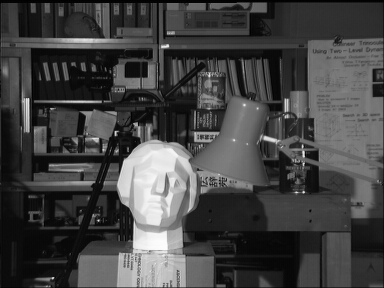
\includegraphics[width=\linewidth]{../data/tsukuba_l.png}} & Tsukuba & 384  & 288 \\[1cm]
 \parbox{2.5cm}{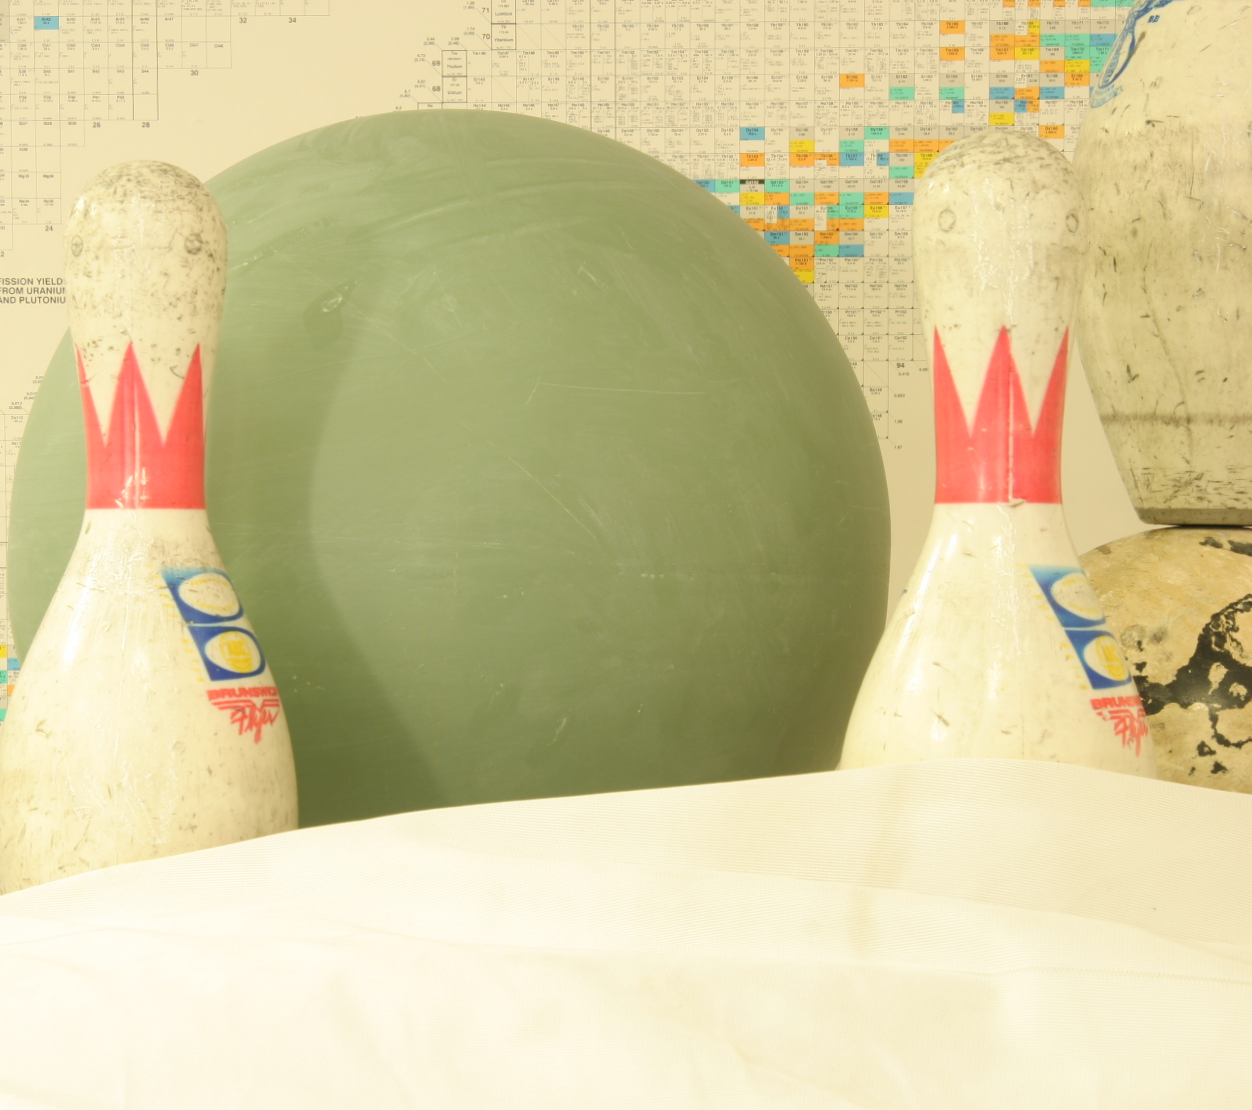
\includegraphics[width=\linewidth]{../data/bowling_l.png}} & Bowling & 1252  & 1110 \\[1cm]
\bottomrule
\end{tabular}
\caption{Datasets used in our tests.}
\label{dataset_table}
\end{table}

\section{Performance Results}

Two computers with different hardware were used for testing. The first, \textbf{Computer 1} has the following specs:

\begin{itemize}
	\item Intel Core i7-3770 CPU (4 cores, 8 threads)
	\item NVIDIA GT 640 graphics card
	\item 16 GB of 1600 MHz DDR3 RAM
	\item WDC WD10EZRX HDD
\end{itemize} 

The second, \textbf{Computer 2} has the following specifications:

\begin{itemize}
	\item Intel Core i7-4930K CPU (6 cores, 12 threads)
	\item NVIDIA GTX 780Ti graphics card
	\item 16 GB of 2133 MHz DDR3 RAM
	\item WD Caviar Black HDD
\end{itemize} 

The operating system used to run the tests was Windows 7 x64, with the VC{}\verb!++! v110 compiler.

\begin{figure}[h]
	\centering
	\subfigure[Computer 1]{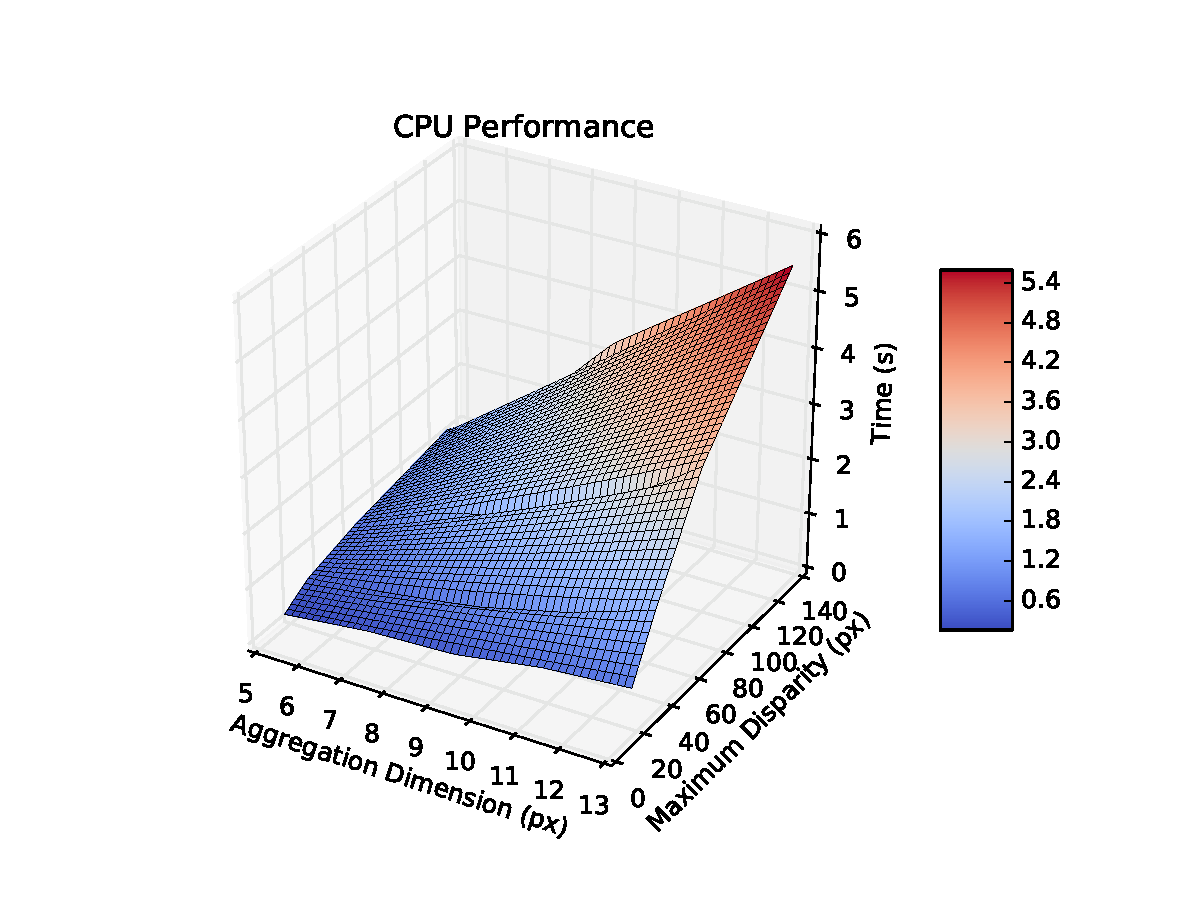
\includegraphics[width=0.49\textwidth]{figures/tsu_perf_cpu_3d_1.pdf}} \hfill
	\subfigure[Computer 2]{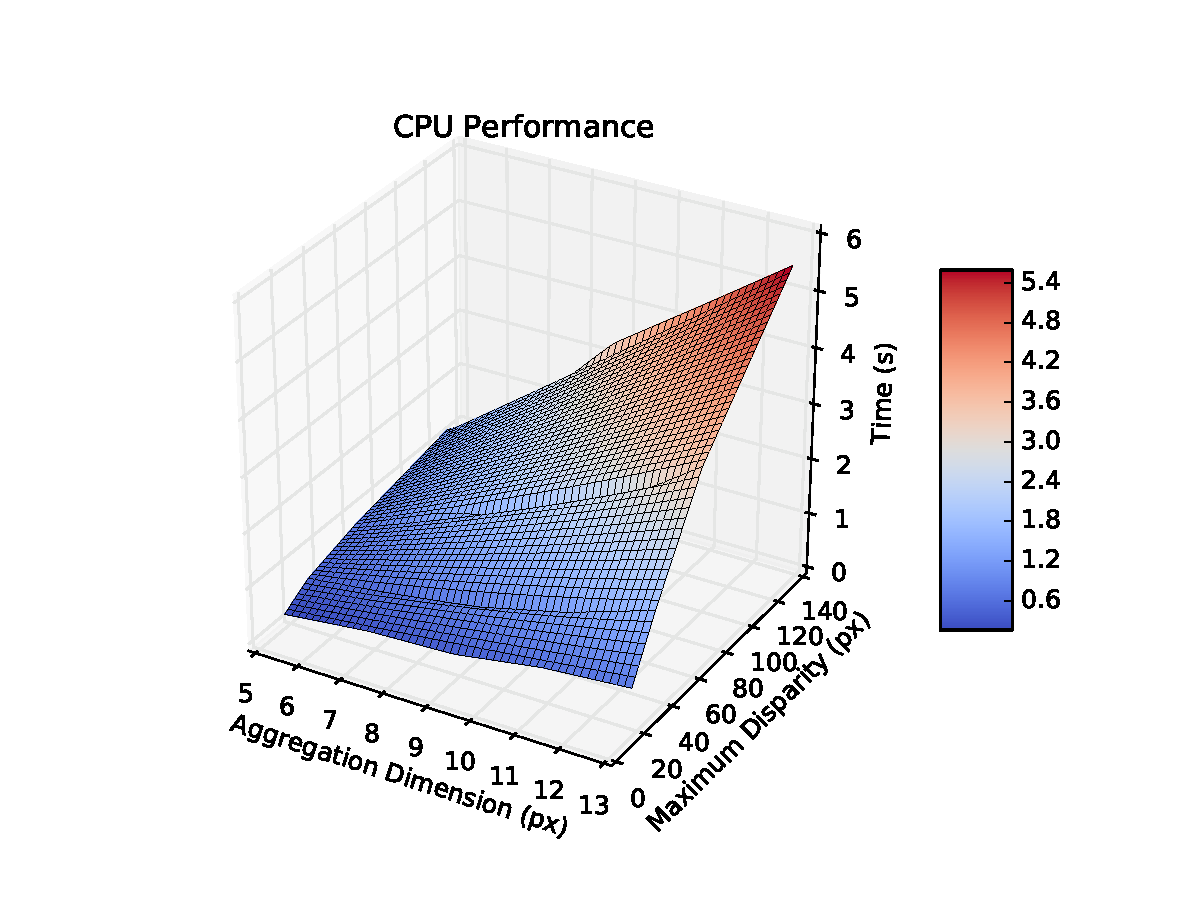
\includegraphics[width=0.49\textwidth]{figures/tsu_perf_cpu_3d_1.pdf}} \hfill
	\caption{CPU performance results for the Tsukuba dataset.} \label{perf_cpu_3d}
\end{figure} 

\begin{figure}[h]
	\centering
	\subfigure[Computer 1]{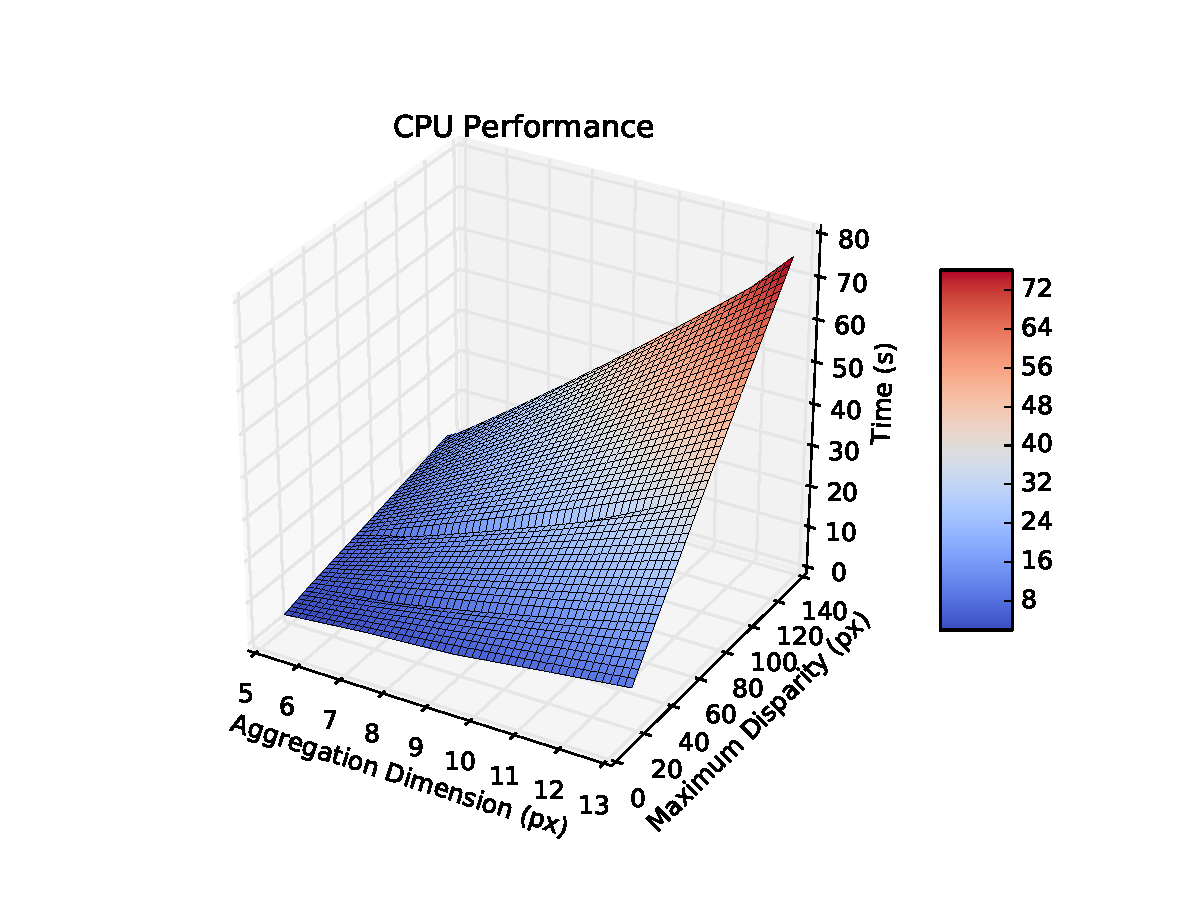
\includegraphics[width=0.49\textwidth]{figures/bow_perf_cpu_3d_1.pdf}} \hfill
	\subfigure[Computer 2]{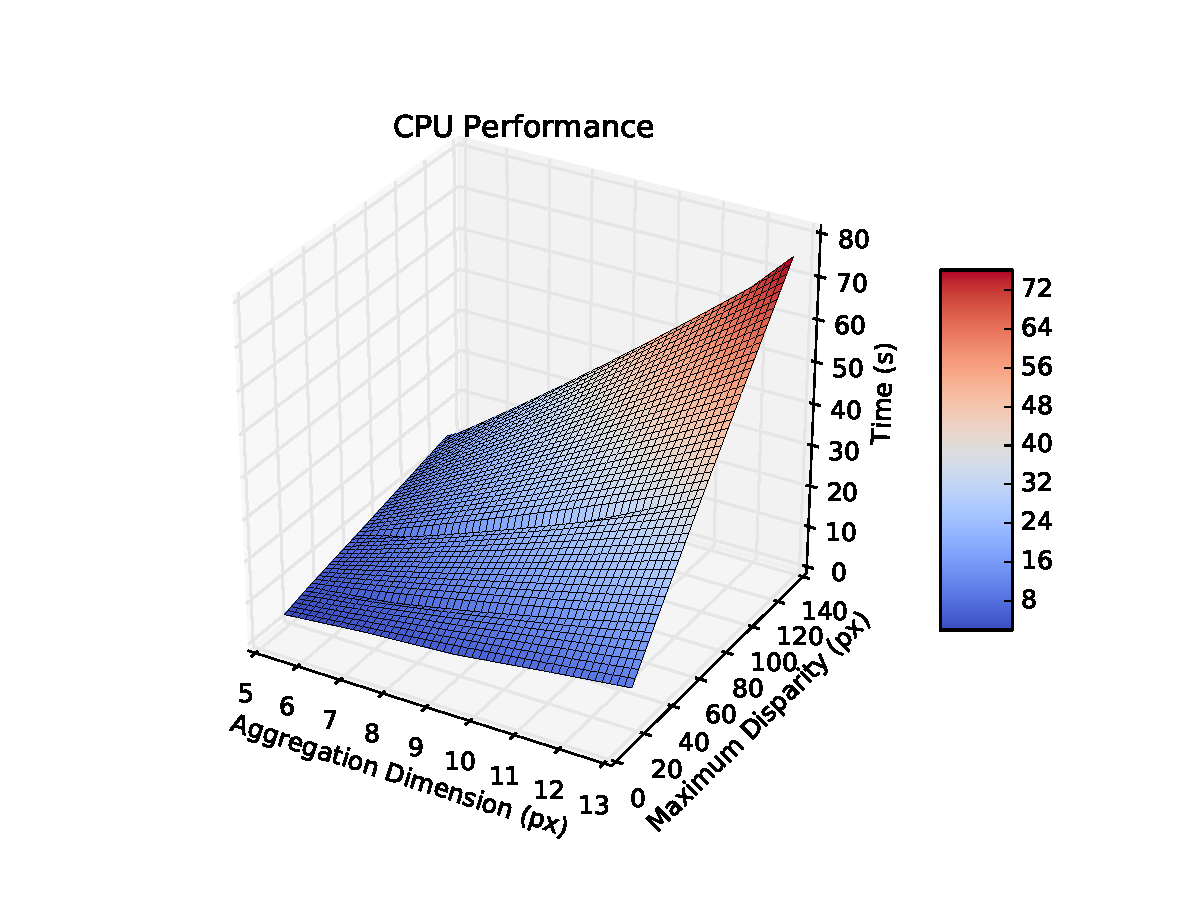
\includegraphics[width=0.49\textwidth]{figures/bow_perf_cpu_3d_1.pdf}} \hfill
	\caption{CPU performance results for the Bowling dataset.} \label{perf_cpu_3d_bow}
\end{figure} 

\begin{figure}[h]
	\centering
	\subfigure[Computer 1]{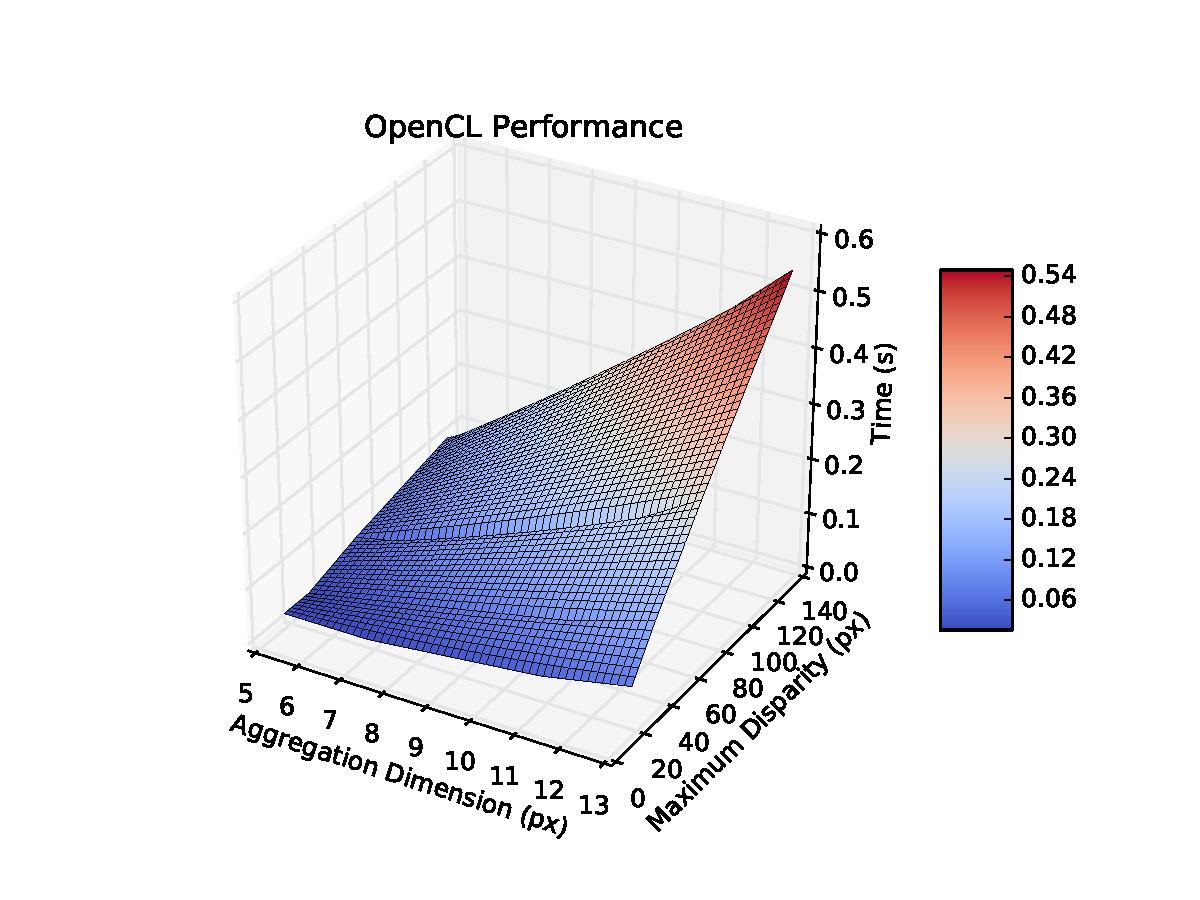
\includegraphics[width=0.49\textwidth]{figures/tsu_perf_ocl_3d_1.pdf}} \hfill
	\subfigure[Computer 2]{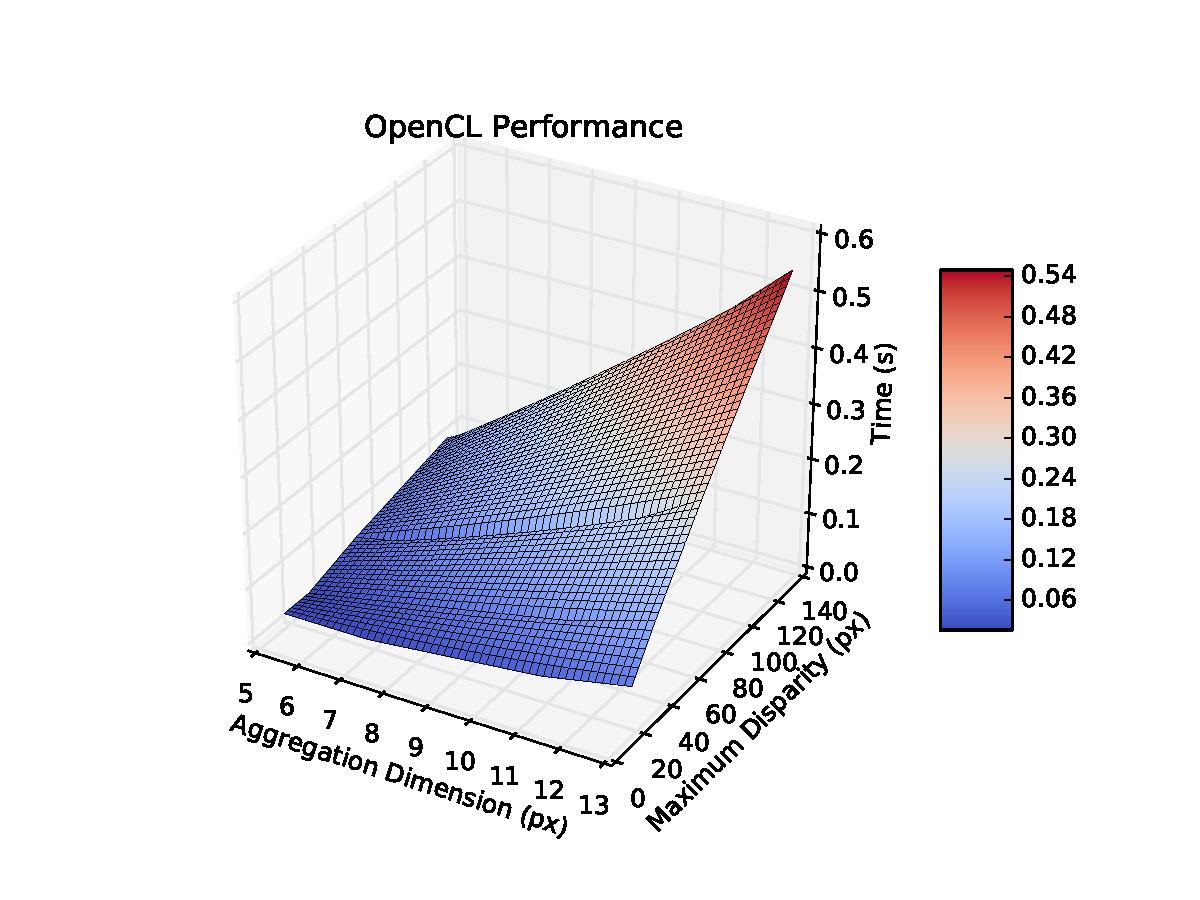
\includegraphics[width=0.49\textwidth]{figures/tsu_perf_ocl_3d_1.pdf}} \hfill
	\caption{OpenCL performance results for the Tsukuba dataset.} \label{perf_ocl_3d}
\end{figure} 

\begin{figure}[h]
	\centering
	\subfigure[Computer 1]{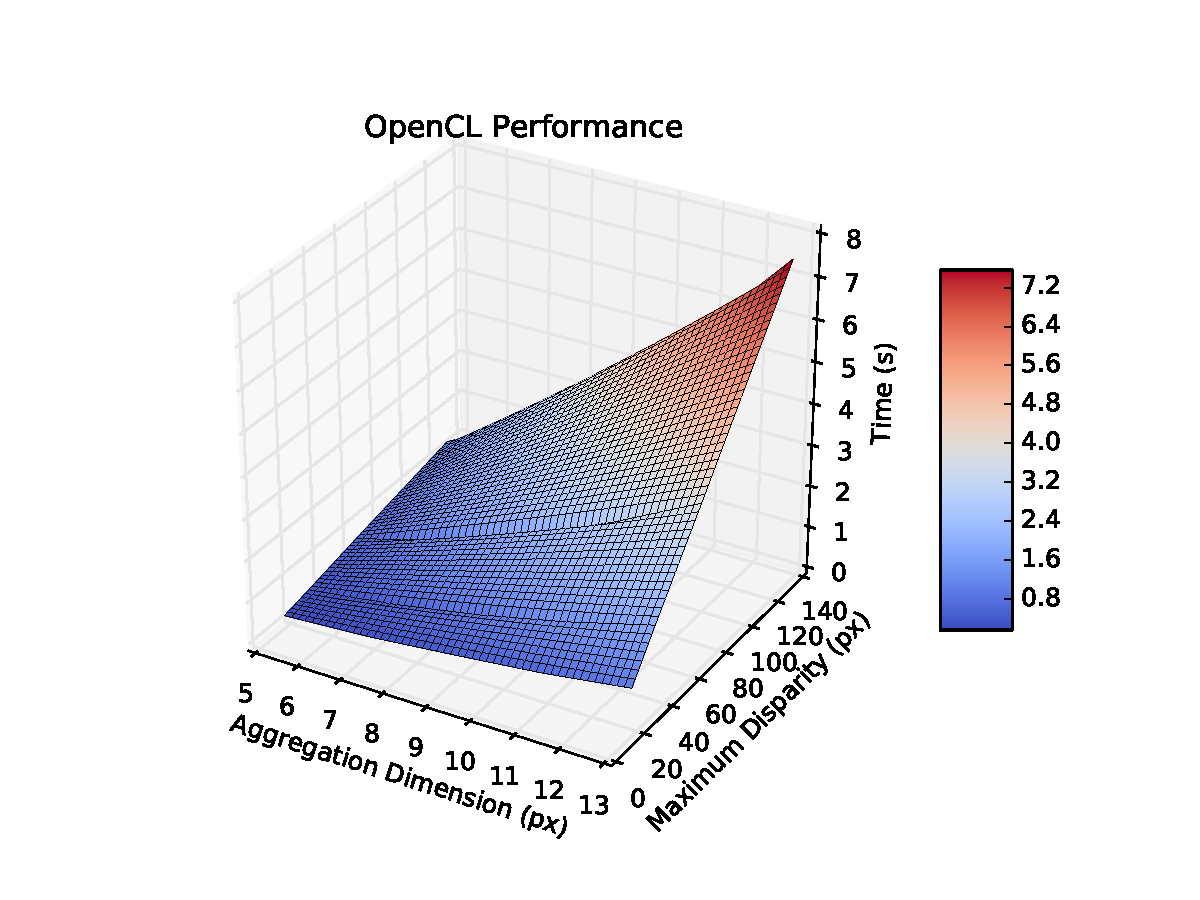
\includegraphics[width=0.49\textwidth]{figures/bow_perf_ocl_3d_1.pdf}} \hfill
	\subfigure[Computer 2]{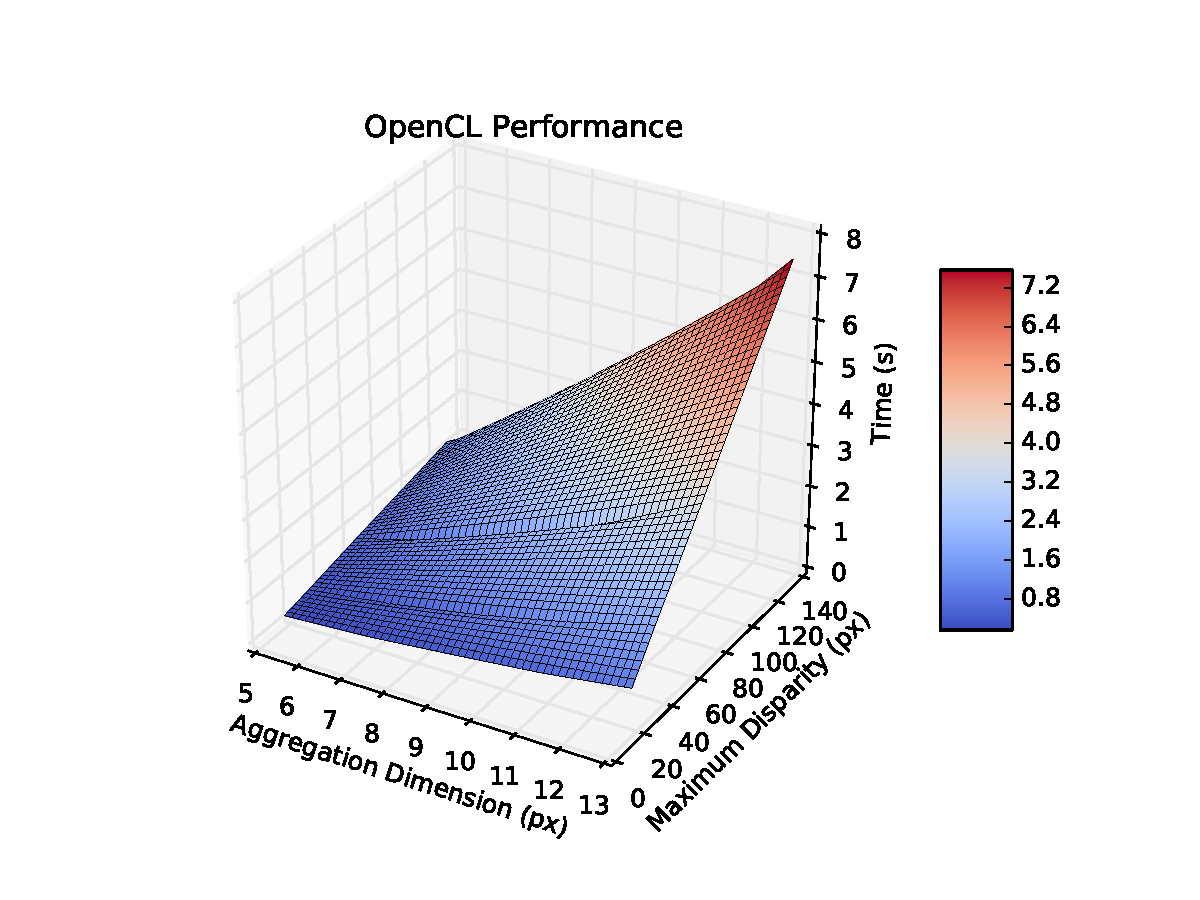
\includegraphics[width=0.49\textwidth]{figures/bow_perf_ocl_3d_1.pdf}} \hfill
	\caption{OpenCL performance results for the Bowling dataset.} \label{perf_ocl_3d_bow}
\end{figure} 

\begin{figure}[h]
	\centering
	\subfigure[Computer 1]{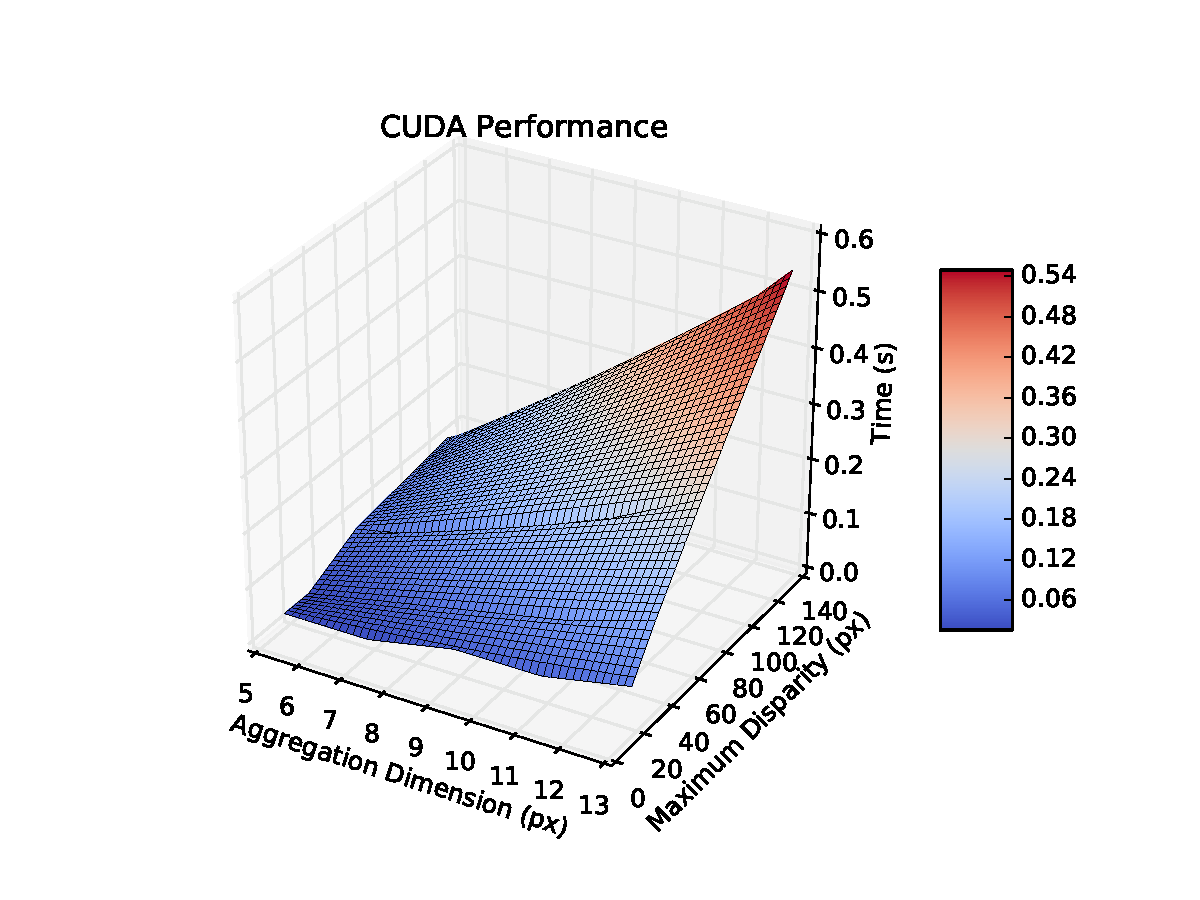
\includegraphics[width=0.49\textwidth]{figures/tsu_perf_cuda_3d_1.pdf}} \hfill
	\subfigure[Computer 2]{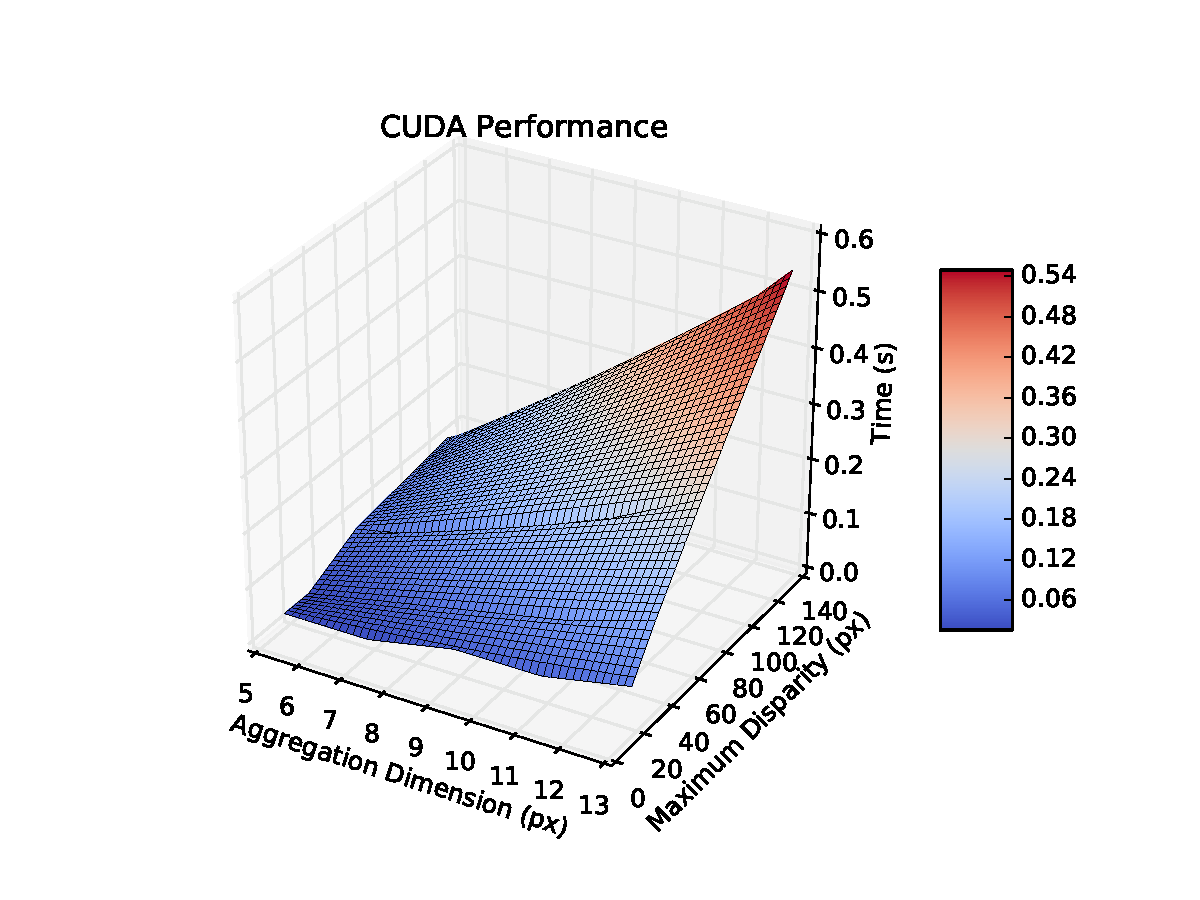
\includegraphics[width=0.49\textwidth]{figures/tsu_perf_cuda_3d_1.pdf}} \hfill
	\caption{CUDA performance results for the Tsukuba dataset.} \label{perf_cuda_3d}
\end{figure} 

\begin{figure}[h]
	\centering
	\subfigure[Computer 1]{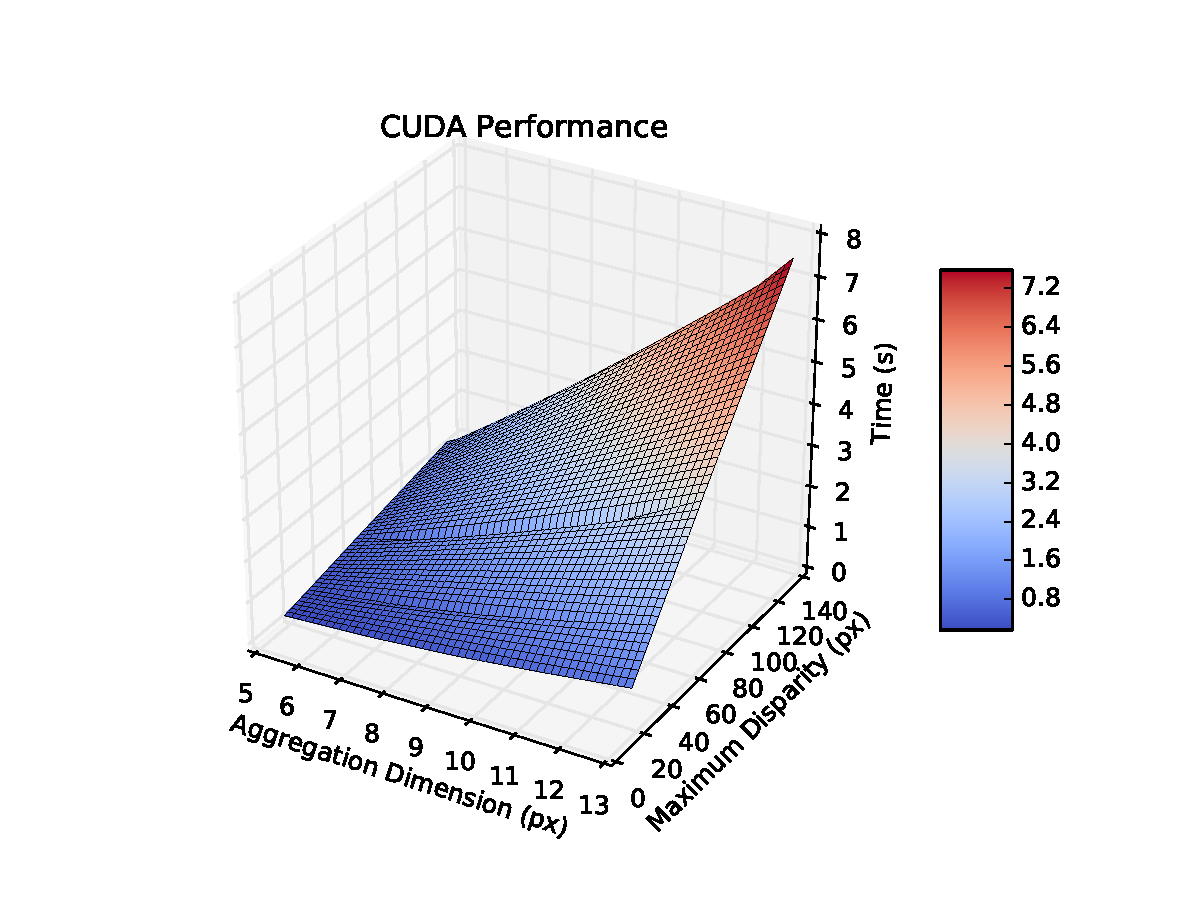
\includegraphics[width=0.49\textwidth]{figures/bow_perf_cuda_3d_1.pdf}} \hfill
	\subfigure[Computer 2]{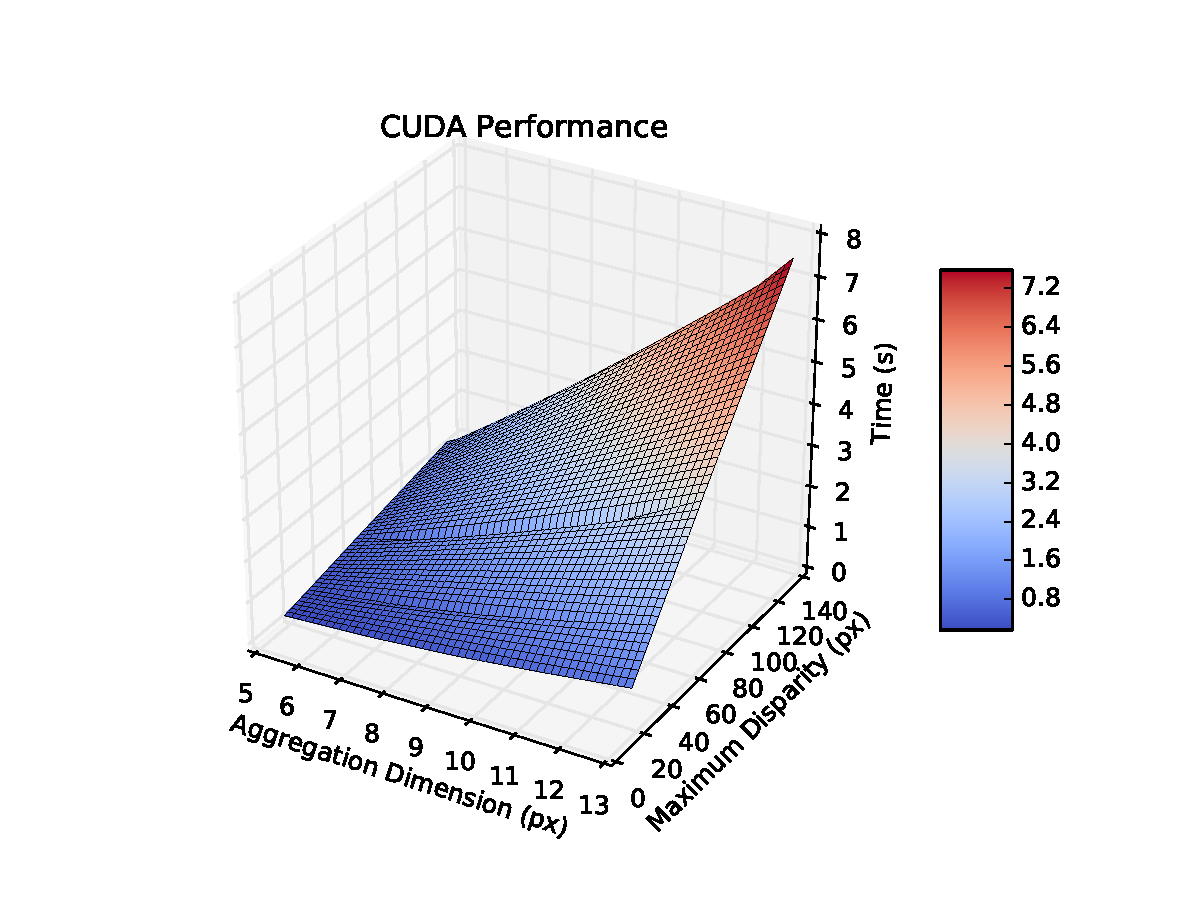
\includegraphics[width=0.49\textwidth]{figures/bow_perf_cuda_3d_1.pdf}} \hfill
	\caption{CUDA performance results for the Bowling dataset.} \label{perf_cuda_3d_bow}
\end{figure} 

\section{Experimental Results}

\begin{figure}[h]
	\centering
	\subfigure[Resulting depth map]{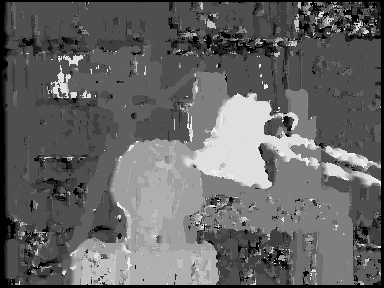
\includegraphics[width=0.49\textwidth]{figures/tsukuba_dm_5_16.jpg}} \hfill
	\subfigure[Ground truth depth map]{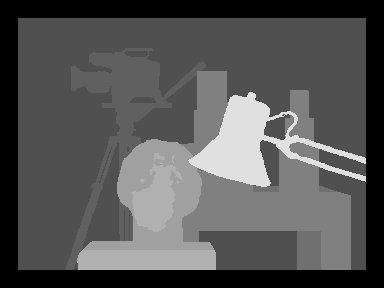
\includegraphics[width=0.49\textwidth]{figures/tsukuba_o_d.jpg}} \hfill
	\caption{Depth map obtained with a maximum disparity of 16 and an aggregation window of 5 in the Tsukuba dataset.} \label{tsukuba_depth_map_1}
\end{figure} 

In order to test the implemented algorithm, we have processed the test images with GCVL. The first results obtained were the depth maps of the Tsukuba dataset, they can be seen in \autoref{tsukuba_depth_map_1} and \autoref{tsukuba_depth_map_2}.

\begin{figure}[h]
	\centering
	\subfigure[Resulting depth map]{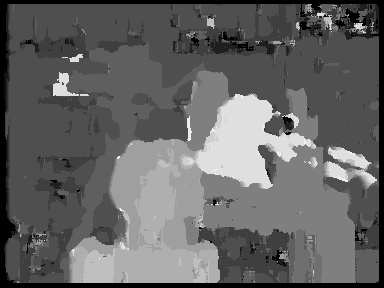
\includegraphics[width=0.49\textwidth]{figures/tsukuba_dm_9_16.jpg}} \hfill
		\subfigure[Ground truth depth map]{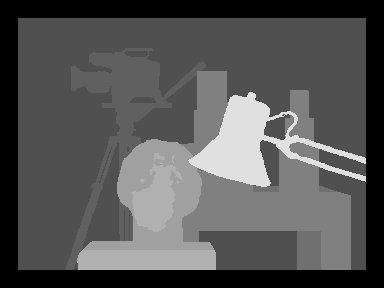
\includegraphics[width=0.49\textwidth]{figures/tsukuba_o_d.jpg}} \hfill
	\caption{Depth map obtained with a maximum disparity of 16 and an aggregation window of 9 in the Tsukuba dataset.} \label{tsukuba_depth_map_2}
\end{figure} 

As we can see in the tests, as we increase the aggregation window size, the depth map becomes smoother. The main drawback when increasing this parameter, is that a loss of detail occurs, since the pixel window compared is bigger and the estimation is more statistically robust but less coarse.

\begin{figure}[h]
	\centering
	\subfigure[Bowling dataset]{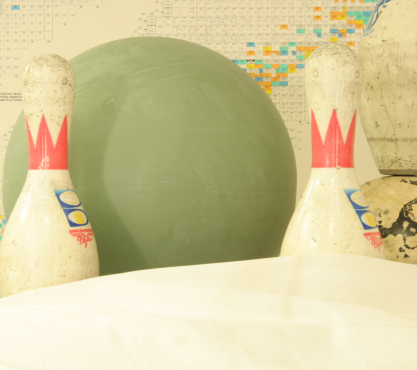
\includegraphics[width=0.49\textwidth]{figures/bowling.png}} \hfill
		\subfigure[Textureless map]{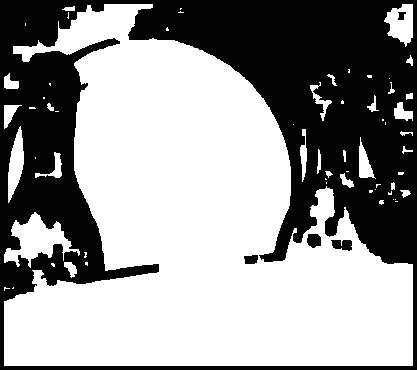
\includegraphics[width=0.49\textwidth]{figures/bowling-textureless-map.png}} \hfill
	\caption{Textureless map of the Bowling dataset, pixels marked as white are low-texture regions.} \label{textureless_regions}
\end{figure}

Moreover, we can see that there are some artifacts in the obtained depth maps. The first reason why these artifacts occur is because of half-occluded (objects in the scene in one image, and not in the other) pixels in the final disparity map. There can also be occluded regions in the left and right images. In addition, there can be regions where there is little or no texture in the scene (a good example of this can be seen in the bowling ball of the Bowling dataset). These can be defined in \cite{scharstein2002taxonomy} as regions where the squared horizontal intensity gradient averaged over a square window of a given size is below a given threshold (see \autoref{textureless_regions}).

\begin{figure}[h]
	\centering
	\subfigure[Resulting depth map]{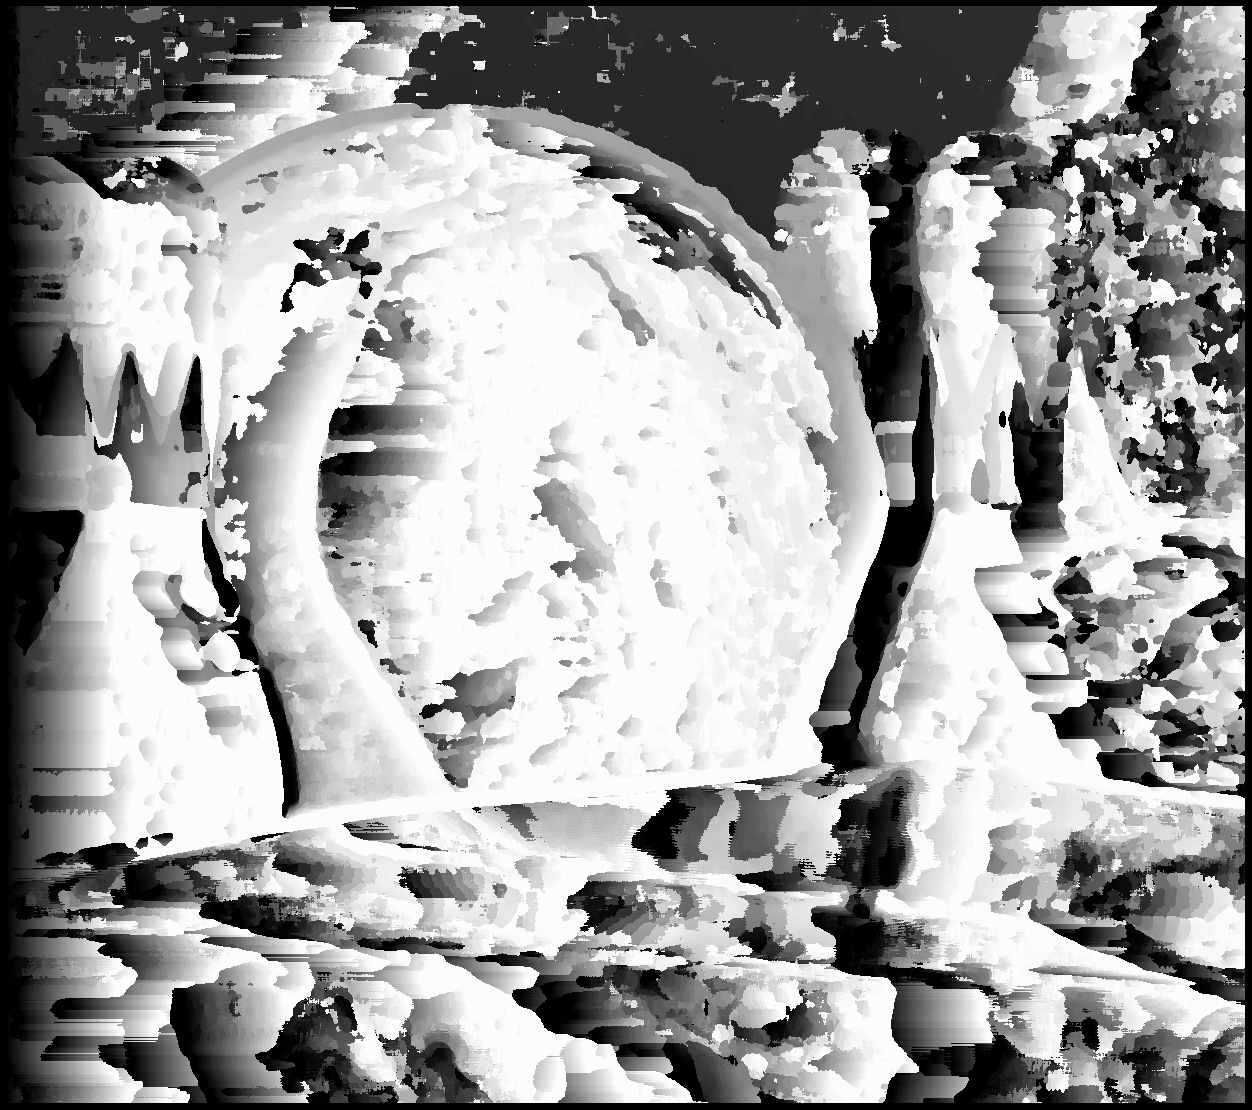
\includegraphics[width=0.49\textwidth]{figures/bowling_dm_13_100.jpg}} \hfill
	\subfigure[Ground truth depth map]{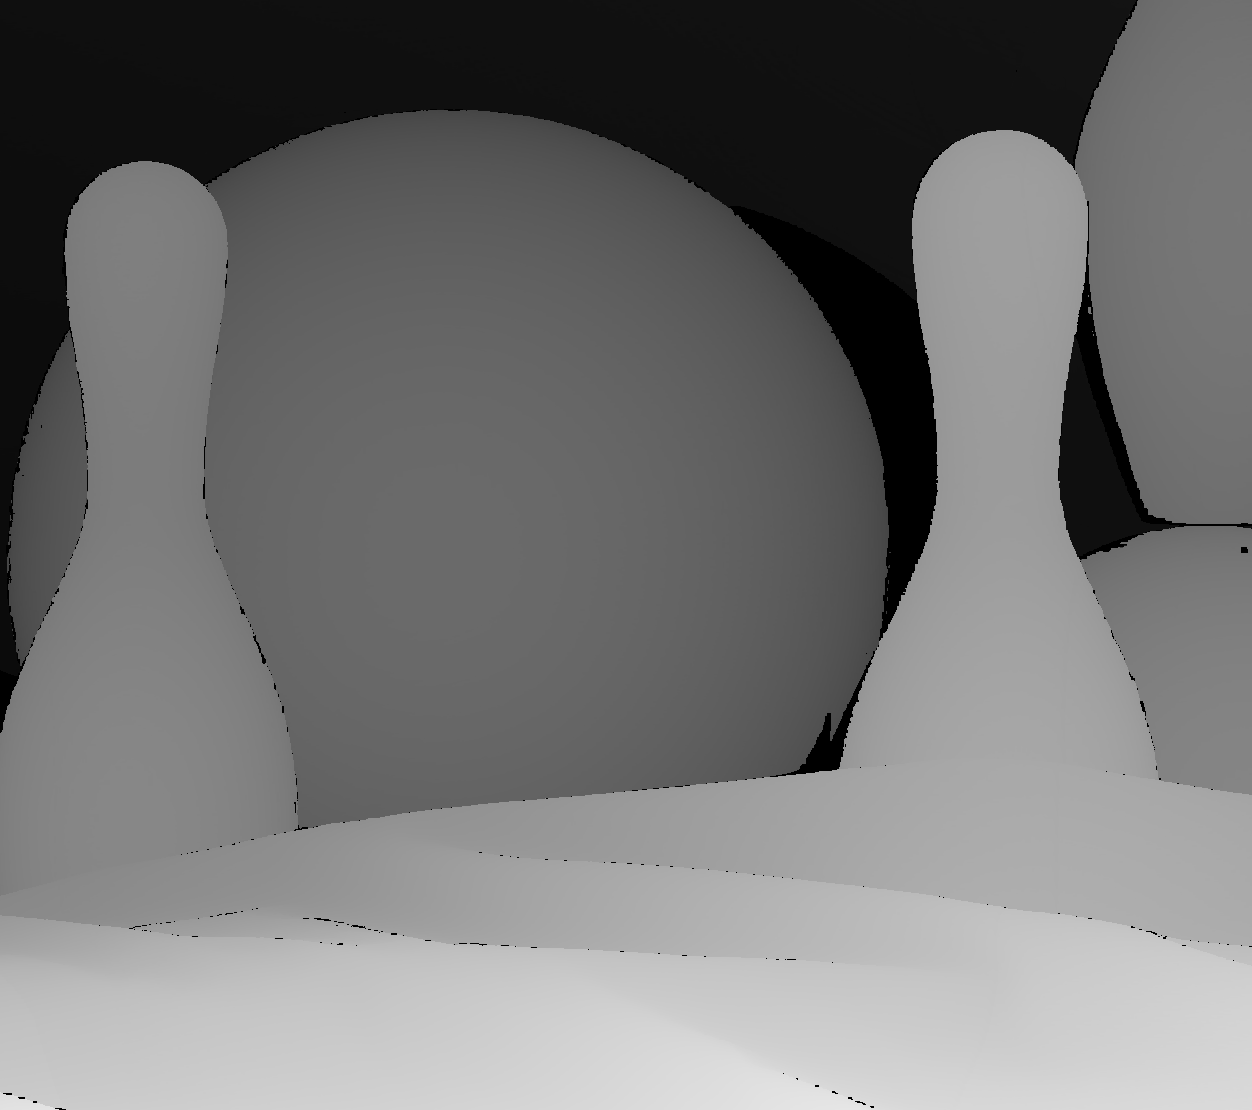
\includegraphics[width=0.49\textwidth]{figures/bowling_o_d.png}} \hfill
	\caption{Depth map obtained with a maximum disparity of 100 and an aggregation window of 13 in the Bowling dataset.} \label{bowling_depth_map_1}
\end{figure}

We can see some of the aforementioned effects in the Second results obtained using the Bowling dataset. The resulting depth maps can be viewed in \autoref{bowling_depth_map_1} and \autoref{bowling_depth_map_2}.

\begin{figure}[h]
	\centering
	\subfigure[Resulting depth map]{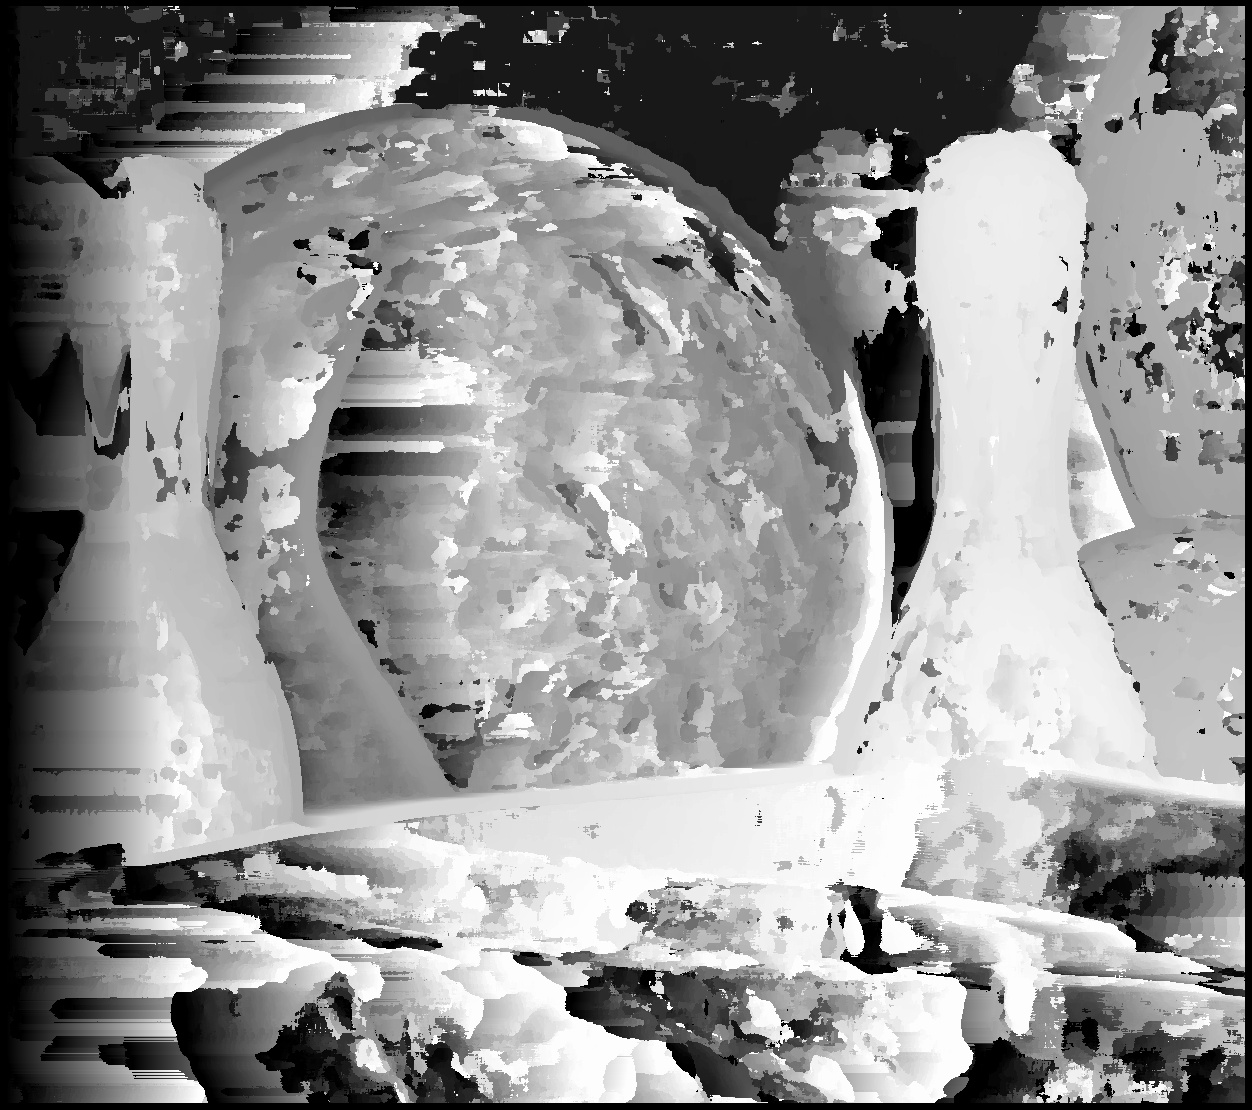
\includegraphics[width=0.49\textwidth]{figures/bowling_dm_13_170.jpg}} \hfill
	\subfigure[Ground truth depth map]{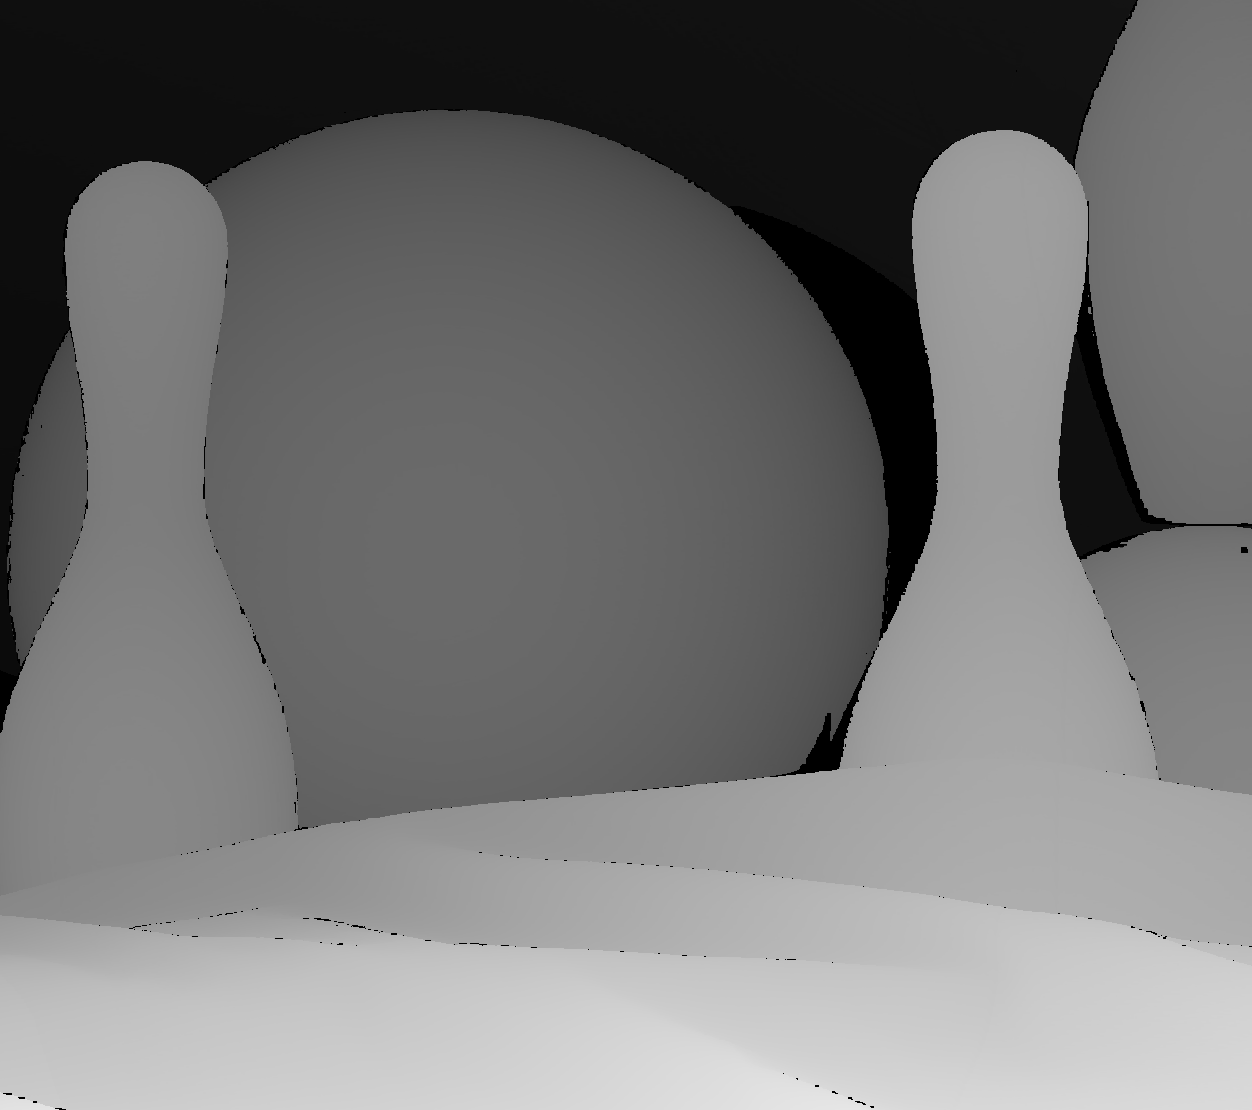
\includegraphics[width=0.49\textwidth]{figures/bowling_o_d.png}} \hfill
	\caption{Depth map obtained with a maximum disparity of 170 and an aggregation window of 13 in the Bowling dataset.} \label{bowling_depth_map_2}
\end{figure}

In the first test we have seen how the aggregation window size influences the smoothness of the disparity map, now we have used a different maximum disparity in each case. If we choose a lower maximum disparity, the algorithm will be faster, but one runs the risk of not finding the corresponding window in the right image. 

In our datasets from the Middlebury Stereo's website, then the answer is simple. The maximum disparity value is the maximum value of the pixel in the ground truth map, divided by the scale factor. If the user has a stereo vision set-up taking real-world imagery, then we will have to do a bit of math to calculate the values. The first equation that we will use is the following:

\begin{equation}
r = \frac{bf}{Nx}
\end{equation}

Being $r$ the range of the object that we are trying to compute, $b$ the distance between the centers of the two cameras, $f$ the focal length of the image sensor, $x$ the pixel size of the sensor and $N$ the maximum disparity value.

Another aspect to account for is the uncertainty in detecting objects at a certain range and the actual range itself. The equation that relates these two variables is the next:

\begin{equation}
\Delta r = \left ( \frac{r^2}{bf}\right)x\Delta N
\end{equation}

Being $\Delta r$ the uncertainty in detecting the object at a certain range and $\Delta N$ the change in disparity value. This means, that for a certain range, we will have some uncertainty in the obtained measurements. For more information the user can check \cite{khaleghi2008improved,khaleghi2008new}.
  